\chapter{Experiments}%
\label{ch:experiments}%
\marginnote{All code can be found under: \url{github.com/morris-frank/unsupervised-source-separation/} (MIT)}%
As we have laid out in the previous chapter our method mainly depends on the quality of the learned source priors. Remember we learn the source priors independently for each source channel. In the VAE-style approach, we learn the posterior for each search with the KL-divergence from the respective prior. In the sampling approach, we optimize the separation solutions under the source priors. Therefore we need the prior models to fulfill some qualities. First, the learned distributions have to generalize, as in both approaches the separation predictions have to be findable in the prior distributions. Second, the priors have to be smooth, so that the priors are capable of assigning lower to higher likelihood to samples that are more true to in-distributions samples. And third, the prior models have to be discriminative. They are trained only on samples of their respective class, but in the separation process, they have to able to discriminate the other signals in the mix from their in-distribution.

\section{Datasets}
We will be working on two datasets. First, a simplified Toy dataset which is made of simple generated signals and second the \texttt{musdb18} dataset which is a widely-used test-set for musical source separation.

\subsection{ToyData}
\begin{marginfigure}[5em]
    \resizebox{\textwidth}{!}{%
        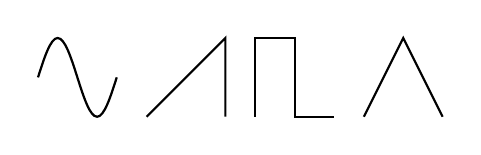
\begin{tikzpicture}
    \node[matrix,thick,column sep=1em,row sep=1em]
    {
        \draw (0,0.5) sin (0.25,1) cos (0.5,0.5) sin (0.75,0) cos (1,0.5); &
        \draw (0,0) -- (1,1) -- (1,0); &
        \draw (0,0) -- (0,1) -- (0.5,1) -- (0.5,0) -- (1,0); &
        \draw (0,0) -- (0.5,1) -- (1,0); \\
    };
\end{tikzpicture}
%
    }%
    \caption{One period of each of the four toy sources: sinus, sawtooth, square and triangle wave.}%
    \label{fig:toy_data}
\end{marginfigure}

We simplify the problem domain to create a toy-like dataset. We randomly generate waves from four simple oscillations: a sine wave, a sawtooth wave, a square wave and a triangle wave; see \cref{fig:toy_data}.  We select the period and phase of each signal in each sample independently and randomly, but fixed for the sample. The frequency is a uniformly picked form the frequency bounds of the 88 keys of an equal-temperament tuned piano (see~\sref{subsec:audio}). The period is also uniformly picked. Given a wave from each source, the mix is computed by simply taking the mean. In our experiments we are gonna model these sources with probability densities, looking especially at the square that will pose a problem, as those only consist of two unique values (\(-1\) and \(1\)). This distribution would simplify the problem too much, therefore we also vary the amplitude of the sampled signals in the uniform range \([0.8, 1.0]\). The signals are sampled with a sampling rate of \(14.700 \si{\Hz}\).

\subsection{musdb18}
Further we use the \texttt{musdb18}~\cite{rafiiMUSDB182017} dataset published for the 2018 Signal Separation Evaluation Campaign~\cite{stoter20182018}. The dataset consists of 150 full songs covering various artists and genres, split into train and test sets sized 100 and 50, respectively. Each track is separated into the four sources \emph{drums}, \emph{bass}, \emph{vocals} and \emph{others}. The \emph{others} source channel contains any remaining set of instruments not categorized under the first three ones. The song files are provided in the Stem audio file format~\cite{nativeinstrumentsStem} and encoded at 44.1kHz. Stem here is terming the provided source channels, we use the terms interchangeably.

The dataset consists of the 100 tracks taken from the DSD100~\cite{SiSEC16} dataset and 46 track out of the MedleyDB~\cite{bittnerMedleyDB2016} dataset. Both dataset contain tracks from a wide range of (western) musical genres, Rock, Pop, Rap, Jazz and Metal. While the upstream data sources provide more fine-grained meta-data, \texttt{musdb18} brings all tracks into the same format and stem splitting as described above.

\begin{marginfigure}[3em]
    \resizebox{\textwidth}{!}{%
        \begin{tikzpicture}
    \node[matrix,thick,column sep=1em,row sep=1em]
    {
        \node (bass)    {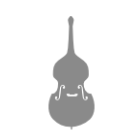
\includegraphics[width=35pt]{../data/images/bass.png}}; &
        \node (drums){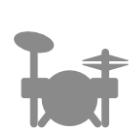
\includegraphics[width=35pt]{../data/images/drums.png}}; &
        \node (voice)  {
\includegraphics[width=35pt]{../data/images/vocals.png}}; &
        \node (other)  {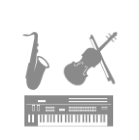
\includegraphics[width=35pt]{../data/images/other.png}}; \\
    };
\end{tikzpicture}
%
    }%
    \caption{The four source channels for the \texttt{musdb18} dataset: bass ,drums, vocals and \I{other}.}%
    \label{fig:musdb_data}
\end{marginfigure}

Next to the separated stems, the dataset provides the original (studio) mix for each song. This mix is not equivalent to the simple linear mixing which we get by taking the mean. Nevertheless, the provided mix diverges only insignificantly from an auto-generated mix, as the original sources are provided in their post-compression, post-mixed form. This means that we can use the original mix and assume it to be reasonably close to the canonical linear mix.

As the songs are real natural songs, they are of different lengths. Our models will different to other recent methods, not be auto-regressive. Thus we sample fixed-length cuts from the songs as training and test samples. For the \texttt{musdb18} data, no pre-processing is applied, as the data already contains the wanted level variability, it spanning different genres and artists.

It is noted that the \texttt{musdb18} dataset while providing a remarkable diverse 10hr of real-world music, is a rather small numbered set of samples. Any data modelling from this set of data will consequently be biased. The dataset specifically is created for the accompanying separation challenge and will not translate to general music modelling.

Also for the \texttt{musdb18} dataset we downsample the signals to \(14.700 \si{\Hz}\).

\section{Prior architectures}

We construct two distinct prior models for the two datasets. All models follow the flow architecture described in \sref{ch:method}. \cref{tab:priors} gives a summary of the networks. Remember the affine transformations are parametrized by WaveNets, consisting of multiple dilated one-dimensional convolutions. We use the gated convolution and skip-connection setup as described in \sref{sec:raw_audio}. We append two extra convolutional layers after the last dilated block with kernel size one and preceding ReLU units, respectively. The last convolutional layer is initialized to zero. This guarantees that at the beginning of training each coupling layer defaults to the identity. All other convolutional weights are initialized with He initalization~\cite{heDelving2015}. The number of features in each convolutional layer is fixed throughout the whole network, as given in the table. All kernels are size \(3\).

\begin{table}
    \begin{tabular}{rccccc}
        \toprule
                                & blocks & flows & layers & kernel size & width   \\
        \midrule
        toy (time)              & 4      & 6     & 10     & 3           & 32      \\
        \texttt{musdb18} (time) & 8      & 6     & 10     & 3           & 48      \\
        \bottomrule
    \end{tabular}%
    \caption{The hyperparameters for the two network architectures. The block is the biggest unit, containing a squeeze operation and \(n_f\) flow blocks. Each flow block contains a activation normalization unit, a affine coupling layer (WaveNet) and a flip operation. The WaveNets cosist of 10 layers each with fixed kernel size and width.}%
    \label{tab:priors}%
\end{table}

\section{Training the priors}
Training of the priors is done in mini-batches with an Adam optimizer~\cite{kingmaAdam2017}. We take random fixed-length samples from the songs/signals in each mini-batch. Each sample is \(16384\) long with is around \(1.1 \si{\sec}\). As all models are fully convolutional the input size is in no way regimented by the architecture, only in so far that we are avoiding padding in the lower layers. The initial learning rate is set to \(1e-4\). The learning rate is decreased with \(\γ=0.6\) and a fixed five-step decrease schedule. The toy model is trained with a batch size of 5 and the \texttt{musdb18} model with a batch size of 2. We train the two prior models first without any added noise for each 150.000. The training curves are shown in \cref{fig:toy_training} and \cref{fig:musdb_training}. As also observed by prior work, the training of deep normalizing flow models behaves unstable.

\begin{figure}
    \includegraphics{toy_noise_0/train.pdf}
    \caption{The negative mean log-likelihood during the training of each ToyData prior. We plot the likelihood and not the loss which include the sum of log-determinant. The instability of the training at the half comes from a restart of training.}%
    \label{fig:toy_training}
\end{figure}

\begin{figure}
    \includegraphics{musdb_noiseless/train.pdf}
    \caption{The negative mean log-likelhood during training of each \texttt{musdb18} prior.}%
    \label{fig:musdb_training}
\end{figure}

For practicality, the priors for all source channels are contained in one model. The PyTorch framework allows for  convolutional layers to be blocked into separate groups. We are not using any operations that are dependent over the batch dimension~\footnote{That would e.g.\ be batch normalization}. We implement the complete flow model in such a grouped way so that the training can be done in parallel on a single GPU while the inference and the gradients for the optimizer updates are independent over the grouped blocks. For that, we also implement the utility functions, squeeze and flip in the same blocked manner.

\section{Testing the priors}
Training of the normalizing flow model combines two objectives: First, we maximize the log-determinant of the \I{non-volume preserving} affine coupling and the activation normalization layers. This guarantees us the invertibility of these transformations. Second, we maximize the likelihood of the projected samples under the chosen target distribution~\footnote{The target distribution is the prior to our prior model. It is set to a factorized Gaussian.}. For the evaluation, we are interested in the mean average likelihood under the target distribution for different in- and out-of-distribution inputs. Remember that the flow gives a bijective mapping between the input and target space~\footnote{necessitated by the invertibility}. For an input of size \(\x \∈ \ℝ^{1\×L}\) the flow returns a latent \(\z \∈ \ℝ^{1\×L}\) of the same size. Each time-point latent \(\z_t\) depends on the  inputs from the receptive field of the flow before and after the respective input \(\x_t\) but is evaluated under the independent margin \(\z_t \sim \N(0,1)\). Because therefore the factorized multivariate Gaussian prior is equivalent to a set of one-dimensional Gaussians, the flow is also not size restricted. All transformations in the network are convolutional and use appropriate padding. \(L\) can be any chosen length. We want to set the input length larger than the receptive field of the network. The latents on either end side of the sample will be based on the larger amount of padded input, while the center values from the sample receive the full receptive field. The size of the receptive field is regimented by the depth and kernel sizes used in the convolutions of the coupling layers and the number of squeeze operations in the blocks (see \cref{fig:squeeze}).

\subsection{Sampling from the priors}
We show an example of sampling from the toy data priors in \cref{fig:toy_time_sample}. It should be unsurprising that the drawn samples are not returning a consistent curve. All the latents are from i.i.d.\ distributions that contribute to the generation of the data output in the bounds of its receptive field. The overlapping receptive fields generate locally consistent curves. This is not a hindrance as our method does not rely on sampling from the priors unconstrained.

\begin{figure}
    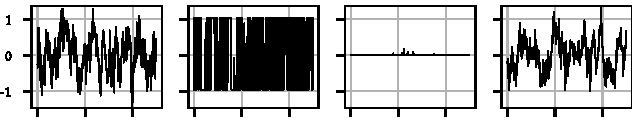
\includegraphics{toy_noise_0/1_samples.pdf}%
    \label{fig:toy_time_sample}%
    \caption{Samples from the prior trained on the toy data.}
\end{figure}

\subsection{Testing cross-likelihood}
In the full model, each prior is used to extract its source channel separately. Through their training, they explicitly contract the density for the positive, in-class examples. During separation, the priors therefore, encounter negative, out-of-distribution samples for the first time. To be useful for separation, the priors have to give a low likelihood to samples from the other classes of the dataset.

\begin{figure}
    \centering
    \begin{subfigure}{0.35\textwidth}
    \includegraphics[width=\textwidth]{toy_noise_0/channels_hm.pdf}%
    \caption{0.0}%
    \label{fig:noiseless_channels_toy}%
\end{subfigure}
\begin{subfigure}{0.35\textwidth}
    \includegraphics[width=\textwidth]{musdb_noiseless/channels_hm.pdf}%
    \caption{0.0}%
    \label{fig:noiseless_channels_musdb}%
\end{subfigure}
%
    \caption{The log-likelihood of each source under each prior for both sets of priors. Notice how for the ToyData we get the diagonal that we are expecting while for the real music the likelihood for every field is high and in the same range. The \I{other} prior assigns the highest likelihoods. For the numerical data see~\cref{tab:cross_likelihood_musdb,tab:cross_likelihood_toy_0}.}%
    \label{fig:noiseless_channels}%
\end{figure}

We test for this by calculating the mean log-likelihood of the test data set under each prior, for each source channel separately. What we anticipate is that the samples from the priors training source are of high likelihood while all other sources are of low likelihood. In \cref{fig:noiseless_channels} (a) we show the source dependent likelihoods for the Toy Data. The in-distribution samples are all of high likelihood while all out-of distribution samples are highly un-likely. The Flow model, therefore, was able to detect out-of-distribution samples while only being trained on in-distribution samples. The estimated densities are discriminative.

When running the same experiment for the \texttt{musdb18} the discriminative power does not hold up, see~\cref{fig:noiseless_channels} (b). All signal sources are about equally likely under each prior density. We hypothesize this stems from the fact that the real musical data is severely more complicated compared to the Toy Data. The Flows model the appearance of sound in general, as the in-class variability of sounds is already high, without knowing anything about the \I{discriminative} differences between the instruments and does not infer the distribution from those features.

Even above that, the results exhibit an additional failing for the \texttt{musdb18} dataset. The third stem in the dataset files \I{other} is filled with a smorgasbord of different instruments. With our training regime, we are implying we can model the sound this set of unrelated instruments with only in-distribution samples with a resulting distribution which is discriminative against another set of unrelated instruments. Intuitively this already fails to be reasonable. Ignoring this difficulty, the priors for\texttt{musdb18} still to fail to be discriminative in the remaining three classes.

We, therefore, continue the investigation of the flow models with the Toy Data.

\section{Noise-conditioning}
We fine-tune the noise-less flow models by continuing the training with added Gaussian noise on the input samples. Fine-tuning~\cite{yosinskiHow2014} the noise-less model instead of retraining the model is considerably cheaper and the noised distribution we want to approximate is close to the noise-free distribution of the initial training. We follow \textcite{jayaramSource2020} in evaluating the noised distribution at variances in 5 steps from 0 to 1, geometrically increasing. The signals with added noise are not capped to the range \([0,1]\) as to not bias the signals towards the bounds of the interval.

We find that fine-tuning converges quickly at between 20.000 and 40.000 steps, see~\cref{fig:toy_noise_conditioned}.

\begin{figure}
    \includegraphics{toy_noise_conditioned/train.pdf}
    \caption{The negative mean log-likelhood during fine-tuning each toy prior with the different levels of noised inputs.}%
    \label{fig:toy_noise_conditioned}
\end{figure}


Conditioning the prior distributions on noised samples is supposed to reduce local peaks in the latent space. \textcite{nalisnickDeep2019} points to the general problem that maximizing the Jacobian of the determinant in the objective of normalizing flows encourages the learned distribution to be sensitive to perturbations of inputs. They warn precisely of assuming anything about the density of a generative model outside of its training data-distribution. Jayaram and Thickstun\footnotemark[\decrvalue{footnote}{1}] experimentally shows that for their source separation method the same problem can be alleviated by fine-tuning on noised samples. Figuratively speaking the Gaussian noise in data space translates to Gaussian smoothing of the peaks in the probability distribution. For our comparatively more complicated models, we want to assess the success of this step.

\begin{figure*}
    \centering
    \foreach\signal in {sin,square,saw,triangle}{
    \begin{subfigure}{0.22\textwidth}
        \includegraphics[width=\textwidth]{noised_noised/\signal_hm.eps}%
        \caption{\signal}%
        \label{fig:noised_noised_\signal}%
    \end{subfigure}
}%
%
    \caption[][\baselineskip]{
        The log likelihood of the test data set with different levels of noise \(\N(0, \σ)\) for the prior models fine-tuned on pertubated data with increasing levels of Gaussian noise. For the numerical data see~\cref{tab:noised_noised_data_sin,tab:noised_noised_data_square,tab:noised_noised_data_saw,tab:noised_noised_data_triangle}.
    }%
    \label{fig:noised_noised}%
\end{figure*}

In \cref{fig:noised_noised} we show the mean average log-likelihood of the test data set with different levels of added noised under the priors fine-tuned with increasing levels of noise. We see that with the noiseless model the likelihood of noised samples quickly decreases with the increasing variance of the noise. Conditioning on a higher variance of noise levels out the likelihood for the lower levels of noise variances. This is not surprising as with the noise conditioning we explicitly model the noised distribution. Consider though the priors conditioned on the noise levels \(0.027\) or \(0.077\). The noised distribution is getting likely for noise levels beyond the conditioned level of noise. Now one might argue that the result, while unexpected, is not prohibitive as the whole point of noise-conditioning is too make `close-to' in-distribution data around as likely as in-distribution data. We argue that our results do show that noise-conditioning the flow distribution is not a pertinent approach to reduce the contractiveness of the latent distribution. Conditioning the noiseless model on low levels of noised data quickly \I{destroys} the previously learned spiked latent distribution.

We show this failing more pronounced in \cref{fig:noised_channels}. Here we plot the mean average likelihood of the different source channels under each prior with widening noise-conditioning. The expectation is to preserve the discriminative power of the different source priors while reducing the sensitivity to noise. The results clearly show that trying to slowly decrease the sensitivity, quickly destroys any discriminative power the generative priors exhibit in the noiseless model.

\begin{figure*}
    \centering
    \begin{subfigure}{0.13\textwidth}
    \includegraphics[width=\textwidth]{toy_noise_0/channels_hm.eps}%
    \caption{0.0}%
    \label{fig:noised_channels_0}%
\end{subfigure}
\foreach\level in {01,027,077,129,359}{
    \begin{subfigure}{0.13\textwidth}
        \includegraphics[width=\textwidth]{toy_noise_\level/channels_hm.eps}%
        \caption{0.\level}%
        \label{fig:noised_channels_\level}%
    \end{subfigure}
}%
%
    \caption[][\baselineskip]{
        The cross-likelihood of the toy source channels under each prior model after conditioning the distribution on different levels of noise. For the numerical data see~\cref{tab:cross_likelihood_toy_01,tab:cross_likelihood_toy_027,tab:cross_likelihood_toy_077,tab:cross_likelihood_toy_129,tab:cross_likelihood_toy_359}.
    }%
    \label{fig:noised_channels}%
\end{figure*}

With the noiseless model \cref{fig:noised_channels} (a) the distribution is discriminative against the samples from the other sources. With increasing noise-conditioning the discriminative power is lost going to (f). The noising of the input data results in the latent distribution to flatten out to the point of not being able to differ between any of the signal channels.
\clearpage%
\section{Random and constant inputs}
\begin{table}
    \begin{tabular}{llrrrr}
\toprule
    &       &      sin &   square &      saw &  triangle \\
value & model &          &          &          &           \\
\midrule
0.0 & 0.0 &  4.8e+00 & -7.0e+02 &  4.4e+00 &   1.8e+00 \\
    & 0.359 & -5.0e-01 & -3.1e+00 &  5.1e+00 &  -2.0e+11 \\
1.0 & 0.0 & -1.5e+01 & -3.6e+03 & -2.7e+06 &  -3.2e+02 \\
    & 0.359 &  2.7e+00 &  4.5e+00 & -2.8e+00 &  -1.1e+01 \\
\bottomrule
\end{tabular}
%
    \caption{The mean log-likelihood of a full receptive field of constant inputs \(\{0,1\}\) for the noise-less and the widest noise-conditioned model.}%
    \label{tab:toy_const}%
\end{table}\vspace{\baselineskip}

Previous works~\cite{sonderbyAmortised2017}\cite{vandenoordParallel2017}\cite{nalisnickDeep2019} have pointed out that generative models tend to assign high likelihood to constant inputs. We examine the same on our Toy Data prior. \cref{tab:toy_const} shows that for the noiseless model the mean data value \(0\) is indeed highly likely, except for the square wave, which we hypothesize stems from the square wave never having that value. Note further that for the noiseless model the maximum input \(1\) is highly unlikely. Noise-conditioning the distribution reverses both values in that the mean value becomes less likely and the maximum value becomes more likely.

\begin{figure}
    \centering
    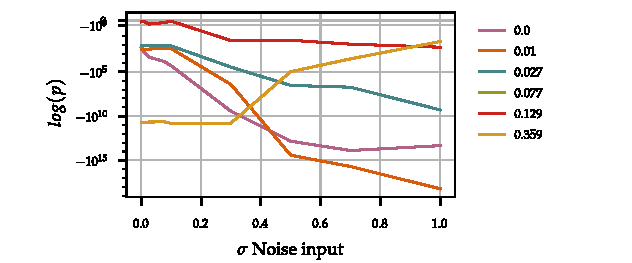
\includegraphics{const_noise_ll.pdf}%
    \caption{The likelihood of Gaussian noise under the Toy prior with increasing variance \(\σ\).}%
    \label{fig:noise_const}%
\end{figure}

On the other hand purely random inputs should be unlikely and decreasing so with higher variance. We plot the relationship between the log-likelihood of Gaussian noise with varying variance under the noiseless and noise-conditioned priors in \cref{fig:noise_const}. We see that for the noiseless model, any amount of noise is highly unlikely. But with wider noise-conditioning this decreases, until with a conditioning of \(0.359\) the effect even reverses.

We read these results to support the previous interpretation that even a small amount of noise fine-tuning can have severe effects on the estimated density. The noiseless model has sharp likelihood peaks around true data, in which even small amounts of noised data are highly unlikely. The noise-conditioning of the flow models flattens these peaks in so far that noise and out-of-distribution samples become highly likely, even at small amounts of added noise.

\section{Langevin sampling}
We tried source separation using the Toy dataset with random mixes and the trained flow priors. As already anticipated with the previous experiments, this is not successful. The noiseless model does not exhibit a smooth manifold which even with the noised gradients of SGLD is optimizable. The noised priors, on the other hand, lost all the discriminative power and therefore it is not possible to modulate the out-of-distribution mix into a true signal by taking (noisy) steps on the prior.
